\documentclass{article}  % Define la clase del documento.

% Paquetes de idioma y codificación
\usepackage[utf8]{inputenc}
\usepackage[T1]{fontenc}
\usepackage[spanish]{babel}  % Ajusta el idioma del documento a español.
\usepackage{tabularx}  % Permite la creación de tablas con ancho ajustable.

% Paquete de geometría para configurar márgenes y tamaño de papel
\usepackage[letterpaper, margin=3cm]{geometry}

% Paquetes de tipografía
\usepackage{mathptmx}    % Usa Times New Roman como fuente.
\usepackage{microtype}   % Mejora la justificación del texto.

% Paquetes para manejo de colores y gráficos
\usepackage{xcolor}      % Define y utiliza colores.
\usepackage{graphicx}    % Permite la inserción de imágenes.
\usepackage{tikz}        % Creación de gráficos vectoriales.

% Configuración de enlaces y referencias cruzadas
\usepackage{hyperref}
\hypersetup{
    colorlinks   = true,
    linkcolor    = black,
    citecolor    = black,
    filecolor    = black,
    urlcolor     = blue
}

\usepackage{media9} % Permite la inserción de multimedia.

% Paquetes para la mejora visual de tablas y figuras
\usepackage{booktabs}    % Para tablas de alta calidad.
\usepackage{float}       % Controla la posición de figuras y tablas.

% Paquete para la personalización de códigos fuente
\usepackage{listings}
\lstset{
    literate=
    {á}{{\'a}}1 {é}{{\'e}}1 {í}{{\'i}}1 {ó}{{\'o}}1 {ú}{{\'u}}1
    {Á}{{\'A}}1 {É}{{\'E}}1 {Í}{{\'I}}1 {Ó}{{\'O}}1 {Ú}{{\'U}}1
    {ñ}{{\~n}}1 {Ñ}{{\~N}}1 {ü}{{\"u}}1 {Ü}{{\"U}}1,
    backgroundcolor=\color{backcolour},
    commentstyle=\color{codegreen},
    keywordstyle=\color{codepurple},
    numberstyle=\tiny\color{codegray},
    stringstyle=\color{red},
    basicstyle=\ttfamily\small,
    breakatwhitespace=false,
    breaklines=true,
    captionpos=b,
    keepspaces=true,
    numbers=left,
    numbersep=5pt,
    showspaces=false,
    showstringspaces=false,
    showtabs=false,
    tabsize=2,
    language=TeX,
    morecomment=[l]\#,
    frame=single,
    rulecolor=\color{black}
}

% Definición de colores al estilo Visual Studio Code
\definecolor{darkblue}{rgb}{0.0, 0.0, 0.55}  % Enlaces
\definecolor{codegreen}{rgb}{0.25, 0.49, 0.48}  % Comentarios
\definecolor{codegray}{rgb}{0.5, 0.5, 0.5}  % Números y anotaciones
\definecolor{codepurple}{rgb}{0.58, 0, 0.82}  % Palabras clave
\definecolor{backcolour}{rgb}{0.95, 0.95, 0.92}  % Fondo de código

% Configuraciones de párrafo y matemáticas
\usepackage{amsmath}
\usepackage{parskip}    % Espaciado entre párrafos.
\usepackage{ragged2e}   % Justificación mejorada.

% Configuración de secciones y encabezados
\usepackage{titlesec}
\titleclass{\part}{top} % Make part like a class
\titleformat{\part}[display]
  {\normalfont\huge\bfseries\centering}{\thepart}{40pt}{\Huge}
\titlespacing*{\part}{0pt}{-60pt}{10pt}
\titleformat{\part}
  {\normalfont\huge\bfseries}{}{0pt}{}

% Asegúrate de usar esto para mantener el estilo en las páginas de las partes
\titleformat{\part}[display]
  {\normalfont\huge\bfseries}{}{0pt}{}
  [\thispagestyle{fancy}] % Aplica el estilo fancy a las páginas de las partes

% Configuración de encabezados y pies de página personalizados
\usepackage{fancyhdr}
\pagestyle{fancy}
\fancyhf{}
\fancyhead[L]{\raisebox{0.20cm}{\textbf{Métodos Computacionales en Obras Civiles}}}
\fancyhead[R]{\raisebox{0.1cm}{
\includegraphics[width=0.25\linewidth]{LOGO_UNIVERSIDAD.jpg}}}
\fancyhead[C]{\rule{\textwidth}{0.6pt}}
\fancyfoot[C]{\rule{\textwidth}{0.6pt}}
\fancyfoot[R]{\raisebox{-1.5\baselineskip}{\thepage}}
\renewcommand{\headrulewidth}{0pt}
\renewcommand{\footrulewidth}{0pt}

% Configuración avanzada de geometría
\geometry{
  top=3.5cm, % Aumenta el espacio en la parte superior para subir el encabezado
  bottom=2.5cm,
  headheight=2.5cm % Aumenta la altura del encabezado si es necesario
}

% Configuracion de bibliografia
\usepackage{natbib}
\bibliographystyle{unsrtnat}  % Puedes cambiarlo por `unsrtnat`, `abbrvnat`, etc.
\usepackage{tabularx} 
\begin{document}
%----------------------------------------------------------------------------------------
% PORTADA
%----------------------------------------------------------------------------------------
\begin{titlepage}%Inicio de la carátula, solo modificar los datos necesarios
\newcommand{\HRule}{\rule{\linewidth}{0.5mm}} 
\center 
%----------------------------------------------------------------------------------------
%	ENCABEZADO
%----------------------------------------------------------------------------------------

\includegraphics[width=10cm]{LOGO_UNIVERSIDAD.jpg}\\ % Si esta plantilla se copio correctamente, va a llevar la imagen del logo de la facultad.OBS: Es necesario incluir el paquete: graphicx
\vspace{3cm}
%----------------------------------------------------------------------------------------
%	SECCION DEL TITULO
%----------------------------------------------------------------------------------------
\HRule \\[0.4cm]
{ \huge \bfseries Entrega 0, Proyecto 2}\\[0.4cm] % Titulo del documento
{ \huge \bfseries Metodos Computacionales en OOCC, IOC 4201}\\[0.4cm] % Titulo del documento
\HRule \\[1.5cm]
 \vspace{5cm}
%----------------------------------------------------------------------------------------
%	SECCION DEL AUTOR
%----------------------------------------------------------------------------------------
\begin{flushright}
    { \textbf{Profesor:}\\
    Patricio Moreno\\
    \vspace{0.2cm}
    \textbf{Ayudante:} \\
    Maximiliano Biasi\\
    \vspace{0.2cm}
    \textbf{Alumno:} \\
    Bernardo Caprile Canala-Echevarría\\

}
\end{flushright}
\vspace{1cm}
%----------------------------------------------------------------------------------------
%	SECCION DE LA FECHA
%----------------------------------------------------------------------------------------
{\large \textbf{\today}}\\[1cm] % El comando \today coloca la fecha del dia, y esto se actualiza con cada compilacion, en caso de querer tener una fecha estatica, reemplazar el \today por la fecha deseada
\end{titlepage}

\newpage
\thispagestyle{empty} % Deshabilita el número de página en la página del índice
\include{resumen}
%----------------------------------------------------------------------------------------
%  INDICE
%----------------------------------------------------------------------------------------
\newpage
\thispagestyle{empty} % Deshabilita el número de página en la página del índice
\tableofcontents
\thispagestyle{plain} % Deshabilita el encabezado en la página del índice
\thispagestyle{empty} % Deshabilita el número de página en la página del índice

\thispagestyle{empty}
\listoffigures 
\thispagestyle{plain} % Deshabilita el encabezado en la página del índice %
\thispagestyle{empty}
\newpage
%----------------------------------------------------------------------------------------
%ACÁ EMPIEZA EL INFORME
\setcounter{page}{1}
\section{Introducción}

\begin{figure}[h]
  \centering
  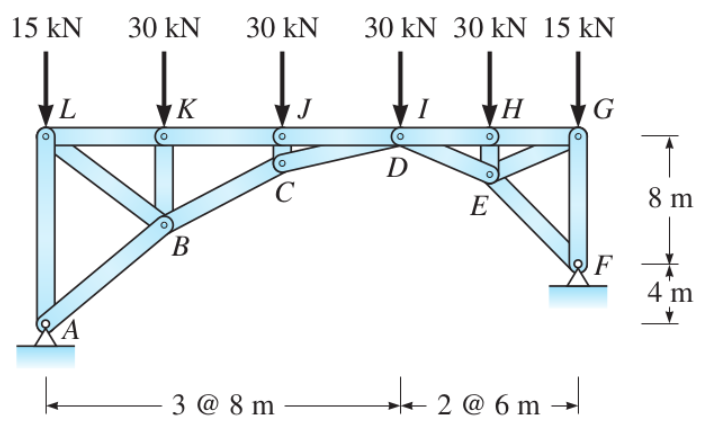
\includegraphics[width=0.8\textwidth]{imagenes/diagrama.png}
  \caption{Enrejado a analizar.}
\end{figure}

\newpage
\section{Método Manual}
Para poder calcular la fuerza en las barras del enrejado, lo que se hizo primero fue calcular la fuerza en las reacciones. Luego, se procedió a calcular la fuerza en cada barra del enrejado con equilibrio de fuerzas en cada nodo. El procedimiento está detallado en el siguiente link: 

\subsection{Resultados Método Manual}
\begin{table}[h!]
  \centering
  \begin{tabular}{|c|c|}
  \hline
  \textbf{Miembro} & \textbf{Fuerza axial (kN)} \\
  \hline
  1  & -15.0   \\
  2  & -89.411 \\
  3  & 0.0     \\
  4  & -0.0    \\
  5  & -30.0   \\
  6  & -71.873 \\
  7  & -0.008  \\
  8  & 0.008   \\
  9  & -30.0   \\
  10 & -64.313 \\
  11 & -0.008  \\
  12 & -0.0    \\
  13 & -70.062 \\
  14 & -30.0   \\
  15 & 0.0     \\
  16 & -0.0    \\
  17 & -86.488 \\
  18 & -15.0   \\
  \hline
  \end{tabular}
  \caption{Fuerzas axiales en cada barra del enrejado.}
  \label{tab:1}
\end{table}
Luego de calcular las fuerzas axiales, se procedió a determinar la geometría de cada barra, junto con su área y módulo de elasticidad. Como se puede observar en la tabla \ref{tab:1} existen dos rangos de fuerzas axiales, el primero que va desde 0 kN hasta 30kN (Barras tipo B) y el segundo que va desde 30kN hasta 89.411kN (Barras tipo A). Los parámetros de las barras se puedes observar en la siguiente tabla:

\begin{table}[h!]
  \centering
  \begin{tabular}{|c|c|c|c|c|}
  \hline
  \textbf{Tipo de barra} & \textbf{Diámetro exterior (mm)} & \textbf{Espesor (mm)} & \textbf{Inercia (mm\(^4\))} & \textbf{Área (mm²)} \\
  \hline
  A  & 150 & 50  & 24,543,692.61 & 15,707.96 \\
  B  & 100 & 30  & 4,783,074.82  & 6,597.34  \\
  \hline
  \end{tabular}
  \caption{Propiedades de las barras tipo A y B}
\end{table}
  
Con estos datos, se procedió a calcular el desplazamiento en el Nodo D.

\newpage
\section{Método desplazamientos virtuales}
Para poder calcular el desplazamiento en el Nodo D, se empleó el método de desplazamientos virtuales. Este método consiste en aplicar una carga unitaria en el nodo que se quiere calcular el desplazamiento y luego calcular la fuerza en las barras. El procedimiento está detallado en el siguiente link:

\subsection{Resultados Método Desplazamientos Virtuales}

Luego de calcular las fuerzas axiales en cada barra, se procedió a calcular el desplazamiento en el Nodo D con la siguiente fórmula:

\begin{equation}
  \delta = \sum \frac{L_i \cdot N_i \cdot n_i}{EA_i}
  \label{eq:1}
\end{equation}

Donde:
\begin{itemize}
  \item \(L\) es la longitud de la barra. (m)
  \item \(N\) es la fuerza axial en la barra. (kN)
  \item \(n\) es la fuerza axial en la barra generada por la fuerza virtual. 
  \item \(EA\) es el producto del módulo de elasticidad y el área de la barra. (kN)
\end{itemize}

Con los datos obtenidos, se obtuvieron los siguientes resultados:

\begin{table}[h]
  \centering
  
  \begin{tabular}{cc}
    \hline
    \textbf{Eje} & \textbf{Desplazamiento (mm)} \\
    \hline
    X & -1.015 \\
    Y & -2.270 \\
    \hline
  \end{tabular}
\end{table}

\newpage
\section{Código en OpenSees.py}
Para poder calcular las fuerzas en cada barra y los desplazamientos del enrejado, se utilizó la librería OpenSeesPy. El código utilizado se encuentra en el siguiente link:

Lo primero que se hizo fue definir los nodos y las barras del enrejado. Luego, se procedió a definir las propiedades de los materiales y las secciones de las barras. Posteriormente, se definieron las restricciones de los apoyos. Finalmente, se procedió a calcular las fuerzas en las barras y los desplazamientos.

\subsection{Resultados Código en OpenSees.py}
\begin{table}[h!]
  \centering
  \begin{tabular}{|c|c|}
  \hline
  \textbf{Miembro} & \textbf{Fuerza axial (kN)} \\
  \hline
  1  & -15.0   \\
  2  & -89.411 \\
  3  & 0.0     \\
  4  & -0.0    \\
  5  & -30.0   \\
  6  & -71.873 \\
  7  & -0.008  \\
  8  & 0.008   \\
  9  & -30.0   \\
  10 & -64.313 \\
  11 & -0.008  \\
  12 & -0.0    \\
  13 & -70.062 \\
  14 & -30.0   \\
  15 & 0.0     \\
  16 & -0.0    \\
  17 & -86.488 \\
  18 & -15.0   \\
  \hline
  \end{tabular}
  \caption{Fuerzas axiales en cada barra del enrejado.}
  \label{tab:2}
\end{table}

\begin{table}[h!]
  \centering
  \begin{tabular}{|c|c|c|}
  \hline
  \textbf{Nodo} & \textbf{ux (mm)} & \textbf{uy (mm)} \\
  \hline
  1  & 0.0    & 0.0    \\
  2  & -1.539 & -0.13  \\
  3  & -1.096 & 0.7    \\
  4  & -1.539 & 0.608  \\
  5  & -1.522 & 1.116  \\
  6  & -1.539 & 1.11   \\
  D  & -1.539 & -3.055 \\
  8  & -0.972 & -1.396 \\
  9  & -1.539 & -1.453 \\
  10 & -1.539 & -0.087 \\
  11 & 0.0    & 0.0    \\
  \hline
  \end{tabular}
  \caption{Desplazamientos en los nodos}
\end{table}

\newpage
Posteriormente, se procedió a plotear el enrejado sin desplazamientos y con desplazamientos aumentados con un factor de 500, para ver de mejor manera los desplazamientos. Los resultados se pueden observar en la siguiente figura:
\begin{figure}[h]
  \centering
  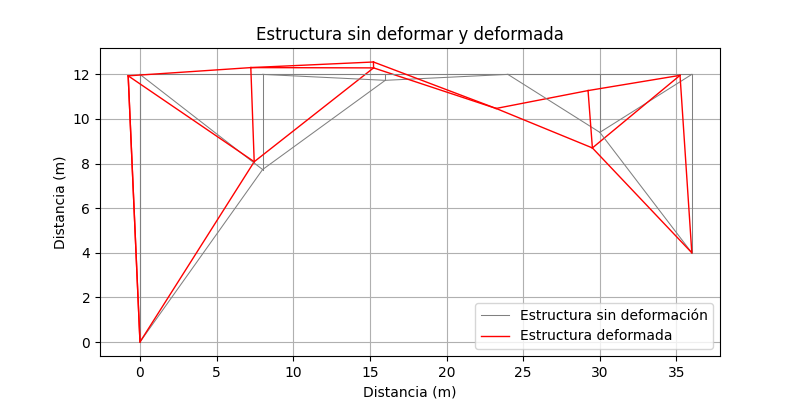
\includegraphics[width=1\textwidth]{imagenes/E0_matplotlib.png}
  \caption{Enrejado sin desplazamientos y con desplazamientos.}
  \label{fig:1}
\end{figure}

\newpage
\section{Análisis de Resultados}
Como se puede observar, los resultados obtenidos con el método manual y programado son prácticamente idénticos. Sin embargo, cuando se compara con el método de desplazamientos virtuales, se observa una diferencia en los desplazamientos en el Nodo D. Esto se puede observar en la siguiente tabla:

\begin{table}[h!]
  \centering
  \begin{tabular}{cccc}
  \hline
  \textbf{Eje} & \textbf{Método Manual (mm)} & \textbf{ Método Desplazamientos Virtuales (mm)} & \textbf{Error (\%)} \\
  \hline
  X & -1.539 & -1.015 & 34.02\\
  Y & -3.055 & -2.270 & 25.67\\
  \hline
  \end{tabular}
  \caption{Comparación de desplazamientos en el Nodo D.}
\end{table}

Aunque hay una diferencia entre los datos obtenidos con el Método de Desplazamientos Virtuales y el software OpenSees.py, esta diferencia se puede explicar porque, en el método manual de desplazamientos virtuales, es fácil cometer errores. Estos errores pueden surgir al hacer los cálculos manualmente o al interpretar los resultados, lo que genera el margen de error observado. Por lo tanto, aunque los resultados no son exactamente iguales, es probable que la diferencia se deba a imprecisiones propias del cálculo manual.

\newpage

\section{Conclusión}


\end{document}